% answers.tex —— 1964 年·全国卷 · 参考答案与详细解析片段
% 由 tools/generate_projects.py 依来源总账自 1964/1964_数学真题_试题.md + 1964/1964_数学真题_解析正文.md + 1964/1964_数学真题_答案要点.md 生成，勿手改（改源 MD 后重跑）


\begin{answer}
\gksolhead{1}{}

\textbf{题目}：

化简：

\nopagebreak[4]
\[\frac{\sqrt[3]{3^{-\frac32}\left(\frac13\right)^{-3}}}{(\sqrt3-1)^2}\]

\Needspace{4\baselineskip}
\textbf{解析}

原式的根号内先合并同底数幂：

\nopagebreak[4]
\[3^{-\frac32}\left(\frac13\right)^{-3}=3^{-\frac32}3^3=3^{\frac32}\]

所以分子为 $\sqrt3$。又

\nopagebreak[4]
\[\left(\sqrt3-1\right)^2=4-2\sqrt3=2(2-\sqrt3)\]

故

\nopagebreak[4]
\[\frac{\sqrt3}{(\sqrt3-1)^2}=\frac{\sqrt3(\sqrt3+1)^2}{\left[(\sqrt3-1)(\sqrt3+1)\right]^2}=\frac{2\sqrt3+3}{2}\]

\gkanswer{答案：$\dfrac{2\sqrt3+3}{2}$}

\end{answer}
\begin{answer}
\gksolhead{2}{}

\textbf{题目}：

甲、乙二人在河的南岸 $O$ 处，隔河在正北方向有一建筑物 $P$。甲向正东、乙向正西沿河岸而行，甲每分钟比乙多走 $a$ 米。10 分钟后，甲望建筑物 $P$ 在北偏西 $\alpha$ 度，乙望建筑物 $P$ 在北偏东 $\beta$ 度，求 $O$ 与 $P$ 之间的距离。

\Needspace{4\baselineskip}
\textbf{解析}

设 $OP=h$，$OB=x$，则 $OA=x+10a$。从 $A$、$B$ 到 $P$ 的正北方向投影分别为沿河岸的距离，因此

\nopagebreak[4]
\[h\tan\alpha=x+10a,\qquad h\tan\beta=x\]

两式相减得

\nopagebreak[4]
\[h(\tan\alpha-\tan\beta)=10a\]

所以

\nopagebreak[4]
\[OP=h=\frac{10a}{\tan\alpha-\tan\beta}\]
\nopagebreak[4]
\begin{center}% 1964 全国卷第 2 题：河岸测距示意图（矢量重绘）
\begin{tikzpicture}[>=stealth,scale=0.82]
  \draw[->] (-3.2,0) -- (3.2,0) node[below right]{河岸};
  \draw[->] (0,-0.15) -- (0,3.25) node[above]{正北};
  \coordinate (O) at (0,0);
  \coordinate (P) at (0,2.65);
  \coordinate (A) at (2.05,0);
  \coordinate (B) at (-1.25,0);
  \draw[dashed] (B) -- (P) (A) -- (P);
  \draw (B) -- (P) (A) -- (P);
  \fill (O) circle (1.5pt) node[below left] {$O$};
  \fill (P) circle (1.5pt) node[above right] {$P$};
  \fill (A) circle (1.5pt) node[below] {$A$};
  \fill (B) circle (1.5pt) node[below] {$B$};
  \draw[<->] (0,-0.38) -- (1.98,-0.38) node[midway,below] {$x+10a$};
  \draw[<->] (-1.18,-0.67) -- (0,-0.67) node[midway,below] {$x$};
  \draw[<->] (0.22,0.05) -- (0.22,2.58) node[midway,right] {$h$};
  \node at (1.38,1.70) {$\alpha$};
  \node at (-0.73,1.28) {$\beta$};
\end{tikzpicture}
\end{center}
\nopagebreak[4]
\gkanswer{答案：$\dfrac{10a}{\tan\alpha-\tan\beta}$}

\end{answer}
\begin{answer}
\gksolhead{3}{}

\textbf{题目}：

解方程 $x^4+1=0$；并且证明：平面内表示这个方程的根的四个点是一个正方形的顶点。

\Needspace{4\baselineskip}
\textbf{解析}

由 $x^4=-1$，写成极形式为

\nopagebreak[4]
\[x^4=\cos(2k+1)\pi+i\sin(2k+1)\pi\]

取 $k=0,1,2,3$，得到

\nopagebreak[4]
\[x_k=\cos\frac{(2k+1)\pi}{4}+i\sin\frac{(2k+1)\pi}{4}\]

即四个根为

\nopagebreak[4]
\[\frac{\sqrt2}{2}(1+i),\quad \frac{\sqrt2}{2}(-1+i),\quad \frac{\sqrt2}{2}(-1-i),\quad \frac{\sqrt2}{2}(1-i)\]

它们的模都为 $1$，相邻根的辐角相差 $\pi/2$，所以对应点在单位圆上等间隔分布，相邻弦长都为 $\sqrt2$，从而四点构成正方形。
\nopagebreak[4]
\begin{center}% 1964 全国卷第 3 题：x^4+1=0 的四根（矢量重绘）
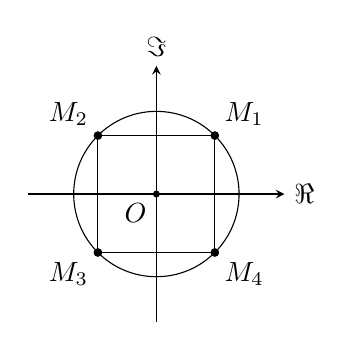
\begin{tikzpicture}[>=stealth,scale=1.05]
  \draw[->] (-1.55,0) -- (1.55,0) node[right] {$\Re$};
  \draw[->] (0,-1.55) -- (0,1.55) node[above] {$\Im$};
  \draw (0,0) circle (1);
  \coordinate (M1) at (0.707,0.707);
  \coordinate (M2) at (-0.707,0.707);
  \coordinate (M3) at (-0.707,-0.707);
  \coordinate (M4) at (0.707,-0.707);
  \draw (M1)--(M2)--(M3)--(M4)--cycle;
  \fill (M1) circle (1.5pt) node[above right] {$M_1$};
  \fill (M2) circle (1.5pt) node[above left] {$M_2$};
  \fill (M3) circle (1.5pt) node[below left] {$M_3$};
  \fill (M4) circle (1.5pt) node[below right] {$M_4$};
  \fill (0,0) circle (1.2pt) node[below left] {$O$};
\end{tikzpicture}
\end{center}
\nopagebreak[4]
\gkanswer{答案：$x=\dfrac{\sqrt2}{2}(1+i),\ \dfrac{\sqrt2}{2}(-1+i),\ \dfrac{\sqrt2}{2}(-1-i),\ \dfrac{\sqrt2}{2}(1-i)$；四点构成正方形。}

\end{answer}
\begin{answer}
\gksolhead{4}{}

\textbf{题目}：

已知 $A$、$B$、$C$ 是三角形的三个内角，求证：

\nopagebreak[4]
\[\cos A=\frac{\sin^2B+\sin^2C-\sin^2A}{2\sin B\sin C}\]

\Needspace{4\baselineskip}
\textbf{解析}

设三角形 $ABC$ 的边长分别为 $a,b,c$，外接圆半径为 $R$。由正弦定理，

\nopagebreak[4]
\[\sin A=\frac{a}{2R},\qquad \sin B=\frac{b}{2R},\qquad \sin C=\frac{c}{2R}\]

于是右端等于

\nopagebreak[4]
\[\frac{\frac{b^2}{4R^2}+\frac{c^2}{4R^2}-\frac{a^2}{4R^2}}{2\cdot\frac{b}{2R}\cdot\frac{c}{2R}}=\frac{b^2+c^2-a^2}{2bc}\]

由余弦定理，$\dfrac{b^2+c^2-a^2}{2bc}=\cos A$，即得所证结论。

\gkanswer{答案：见解析版。}

\end{answer}
\begin{answer}
\gksolhead{5}{}

\textbf{题目}：

已知方程 $x^3+mx^2-3x+n=0$ 的三个根的平方和为 $6$，且知这个方程有两个相等的正根，求 $m$、$n$ 的值。

\Needspace{4\baselineskip}
\textbf{解析}

设两个相等的正根为 $\lambda,\lambda$，另一个根为 $\mu$。由根的平方和与韦达定理，

\nopagebreak[4]
\[2\lambda^2+\mu^2=6,\qquad \lambda^2+2\lambda\mu=-3\]

第二式乘以 $2$ 后与第一式相加，得到

\nopagebreak[4]
\[4\lambda^2+4\lambda\mu+\mu^2=0\]

即 $(2\lambda+\mu)^2=0$，所以 $\mu=-2\lambda$。代入第一式得 $6\lambda^2=6$。因 $\lambda>0$，故 $\lambda=1$，$\mu=-2$。

再次使用韦达定理：

\nopagebreak[4]
\[2\lambda+\mu=-m,\qquad \lambda^2\mu=-n\]

从而 $m=0$，$n=2$。

\gkanswer{答案：$m=0\text{，}n=2$}

\end{answer}
\begin{answer}
\gksolhead{6}{}

\textbf{题目}：

圆台形铁桶的上口半径是 $15$ 厘米，下底半径是 $10$ 厘米，母线长是 $30$ 厘米。将铁桶的侧面沿一条母线剪开铺平，得图中扇面形状的铁片 $ABCD$，求 $A$、$B$ 两点间的距离。
\nopagebreak[4]
\begin{center}% 1964 全国卷第 6 题：圆台与展开扇环（矢量重绘）
\begin{tikzpicture}[>=stealth,scale=0.78]
  % 圆台
  \draw (0,2.25) ellipse (0.78 and 0.18);
  \draw (0,0.25) ellipse (0.52 and 0.13);
  \draw (-0.78,2.25) -- (-0.52,0.25);
  \draw (0.78,2.25) -- (0.52,0.25);
  \draw[dashed] (0,2.25) -- (0,0.25);
  \node at (1.1,2.05) {$15$};
  \node at (0.9,0.45) {$10$};
  \node[right] at (0.64,1.2) {$30$};
  \node at (0,-0.12) {圆台};
  % 扇环
  \draw (3.0,0.25) arc (210:330:2.05);
  \draw (3.0,0.25) arc (210:330:1.25);
  \draw (1.23,-0.78) -- (1.78,-1.65);
  \draw (4.77,-0.78) -- (4.22,-1.65);
  \draw[dashed] (3.0,0.25) -- (1.78,-1.65);
  \draw[dashed] (3.0,0.25) -- (4.22,-1.65);
  \node at (3.0,2.05) {$\theta$};
  \node[above] at (3.0,2.25) {$AB$};
  \node[below] at (3.0,-1.78) {$CD$};
  \node at (3,-2.12) {展开扇环};
\end{tikzpicture}
\end{center}
\nopagebreak[4]
\Needspace{4\baselineskip}
\textbf{解析}

设展开后扇环的内半径为 $x$，则外半径为 $x+30$，圆心角为 $\theta$。上、下底圆周分别成为外、内弧，因而

\nopagebreak[4]
\[30\pi=(x+30)\theta,\qquad 20\pi=x\theta\]

相减得 $30\theta=10\pi$，所以 $\theta=\pi/3$；再由 $x\theta=20\pi$ 得 $x=60$，外半径为 $90$。

弦 $AB$ 对应圆心角 $\pi/3$，故

\nopagebreak[4]
\[AB=2\cdot90\sin\frac{\pi}{6}=90\text{（\text{厘米}）}\]
\nopagebreak[4]
\begin{center}% 1964 全国卷第 6 题：圆台与展开扇环（矢量重绘）
\begin{tikzpicture}[>=stealth,scale=0.78]
  % 圆台
  \draw (0,2.25) ellipse (0.78 and 0.18);
  \draw (0,0.25) ellipse (0.52 and 0.13);
  \draw (-0.78,2.25) -- (-0.52,0.25);
  \draw (0.78,2.25) -- (0.52,0.25);
  \draw[dashed] (0,2.25) -- (0,0.25);
  \node at (1.1,2.05) {$15$};
  \node at (0.9,0.45) {$10$};
  \node[right] at (0.64,1.2) {$30$};
  \node at (0,-0.12) {圆台};
  % 扇环
  \draw (3.0,0.25) arc (210:330:2.05);
  \draw (3.0,0.25) arc (210:330:1.25);
  \draw (1.23,-0.78) -- (1.78,-1.65);
  \draw (4.77,-0.78) -- (4.22,-1.65);
  \draw[dashed] (3.0,0.25) -- (1.78,-1.65);
  \draw[dashed] (3.0,0.25) -- (4.22,-1.65);
  \node at (3.0,2.05) {$\theta$};
  \node[above] at (3.0,2.25) {$AB$};
  \node[below] at (3.0,-1.78) {$CD$};
  \node at (3,-2.12) {展开扇环};
\end{tikzpicture}
\end{center}
\nopagebreak[4]
\gkanswer{答案：$AB=90$ 厘米。}

\end{answer}
\begin{answer}
\gksolhead{7}{}

\textbf{题目}：

$A$、$B$、$C$、$D$ 四个点在平面 $M$ 和平面 $N$ 之外。$A$、$B$、$C$、$D$ 在平面 $M$ 内的射影是 $A_1$、$B_1$、$C_1$、$D_1$，在平面 $N$ 内的射影是 $A_2$、$B_2$、$C_2$、$D_2$。已知 $A_1$、$B_1$、$C_1$、$D_1$ 在一条直线上，$A_2B_2C_2D_2$ 是一个平行四边形，求证 $ABCD$ 也是一个平行四边形。

\Needspace{4\baselineskip}
\textbf{解析}

设 $A_1,B_1,C_1,D_1$ 所在直线为 $l$。过 $l$ 与 $AA_1$ 作平面 $\Pi$。由于 $BB_1\perp M$ 且 $B_1\in\Pi$，又 $BB_1$ 与 $AA_1$ 平行，故 $B\in\Pi$；同理 $C,D\in\Pi$，所以 $ABCD$ 是平面 $\Pi$ 内的四边形。

再看平面 $N$ 的正投影。因为 $AA_2\parallel DD_2$，且 $A_2B_2\parallel D_2C_2$，由两组相交直线分别平行可知，平面 $AA_2B_2$ 与平面 $DD_2C_2$ 平行。它们与平面 $\Pi$ 的交线分别为 $AB$、$CD$，所以 $AB\parallel CD$。同理可得 $BC\parallel AD$，故 $ABCD$ 是平行四边形。
\nopagebreak[4]
\begin{center}% 1964 全国卷第 7 题：两平面射影示意（矢量重绘）
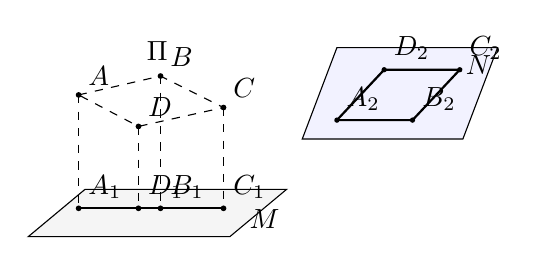
\begin{tikzpicture}[>=stealth,scale=0.8]
  % 平面 M
  \draw[fill=gray!8] (0,0) -- (3.2,0) -- (4.1,0.75) -- (0.9,0.75) -- cycle;
  \node at (3.75,0.28) {$M$};
  % 平面 N
  \draw[fill=blue!5] (4.35,1.55) -- (6.9,1.55) -- (7.45,3.0) -- (4.9,3.0) -- cycle;
  \node at (7.15,2.72) {$N$};
  % Four points in the auxiliary plane and projections to M
  \coordinate (A) at (0.8,2.25);
  \coordinate (B) at (2.1,2.55);
  \coordinate (C) at (3.1,2.05);
  \coordinate (D) at (1.75,1.75);
  \coordinate (A1) at (0.8,0.45);
  \coordinate (B1) at (2.1,0.45);
  \coordinate (C1) at (3.1,0.45);
  \coordinate (D1) at (1.75,0.45);
  \draw[dashed] (A)--(A1) (B)--(B1) (C)--(C1) (D)--(D1);
  \draw[thick] (A1)--(B1)--(C1)--(D1);
  \draw[dashed] (A)--(B)--(C)--(D)--cycle;
  \foreach \p/\name in {A/A,B/B,C/C,D/D,A1/A_1,B1/B_1,C1/C_1,D1/D_1}
    {\fill (\p) circle (1.3pt) node[above right] {$\name$};}
  % Parallelogram on N
  \coordinate (A2) at (4.9,1.85);
  \coordinate (B2) at (6.1,1.85);
  \coordinate (C2) at (6.85,2.65);
  \coordinate (D2) at (5.65,2.65);
  \draw[thick] (A2)--(B2)--(C2)--(D2)--cycle;
  \foreach \p/\name in {A2/A_2,B2/B_2,C2/C_2,D2/D_2}
    {\fill (\p) circle (1.2pt) node[above right] {$\name$};}
  \node at (2.05,2.95) {$\Pi$};
\end{tikzpicture}
\end{center}
\nopagebreak[4]
\gkanswer{答案：见解析版。}

\end{answer}
\begin{answer}
\gksolhead{8}{}

\textbf{题目}：

下图中 $ABCD$ 是正方形，其每边长为 $1$；在正方形内，$\odot O$ 与 $\odot O'$ 互相外切，并且 $\odot O$ 与 $AB$、$AD$ 两边相切，$\odot O'$ 与 $CB$、$CD$ 两边相切。
\nopagebreak[4]
\begin{center}% 1964 全国卷第 8 题：正方形内两圆（矢量重绘）
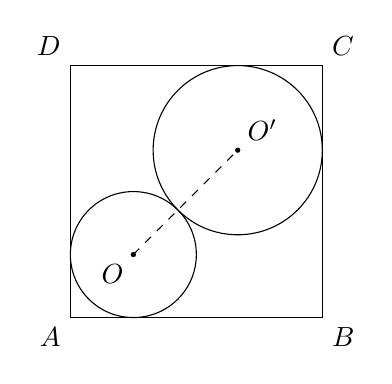
\begin{tikzpicture}[scale=0.8]
  \draw (0,0) rectangle (4,4);
  \node[below left] at (0,0) {$A$};
  \node[below right] at (4,0) {$B$};
  \node[above right] at (4,4) {$C$};
  \node[above left] at (0,4) {$D$};
  \draw (1,1) circle (1);
  \draw (2.657,2.657) circle (1.343);
  \fill (1,1) circle (1.2pt) node[below left] {$O$};
  \fill (2.657,2.657) circle (1.2pt) node[above right] {$O'$};
  \draw[dashed] (1,1) -- (2.657,2.657);
\end{tikzpicture}
\end{center}
\nopagebreak[4]
（1） 求这两圆半径之和。

（2） 当两圆半径各多么长时，两圆面积之和最小？当半径各多么长时，面积之和最大？证明你的结论。

\textbf{附加题}

\begin{itemize}
\item \textbf{附加题（1）} 如果把第 8 题中的正方形改成矩形，你能得到什么结果？为什么？
\end{itemize}

\begin{itemize}
\item \textbf{附加题（2）} 如果把第 8 题中的正方形改成棱长为 $1$ 的正方体，把圆改成球，你能得到什么结果？为什么？
\end{itemize}

\Needspace{4\baselineskip}
\textbf{解析}

\gksubpart{（1）求半径之和}

设两圆半径分别为 $r,r'$，令 $s=r+r'$。以正方形左下角为原点，则两圆心可表示为 $(r,r)$ 与 $(1-r',1-r')$。外切条件给出

\nopagebreak[4]
\[\sqrt2(1-r-r')=r+r'\]

所以

\nopagebreak[4]
\[s=\sqrt2(1-s),\qquad s=\frac{\sqrt2}{1+\sqrt2}=2-\sqrt2\]

\gksubpart{（2）面积和的最值}

两圆均在正方形内，故 $0<r,r'\leqslant\frac12$。面积和为

\nopagebreak[4]
\[S=\pi(r^2+r'^2)=\pi(s^2-2rr')\]

在 $r+r'=s$ 固定时，$rr'$ 在 $r=r'=s/2$ 时最大，因此面积和最小，且

\nopagebreak[4]
\[r=r'=\frac{2-\sqrt2}{2},\qquad S_{\min}=\pi(3-2\sqrt2)\]

在约束 $0<r,r'\leqslant1/2$ 下，$r^2+r'^2$ 在边界处最大。于是一个半径取 $1/2$，另一个取 $s-1/2=3/2-\sqrt2$，故

\nopagebreak[4]
\[\{r,r'\}=\left\{\frac12,\frac32-\sqrt2\right\},\qquad S_{\max}=\pi\left(\frac92-3\sqrt2\right)\]
\nopagebreak[4]
\begin{center}% 1964 全国卷第 8 题：面积和最小时两圆等半径（矢量重绘）
\begin{tikzpicture}[scale=0.8]
  \draw (0,0) rectangle (4,4);
  \draw (1.172,1.172) circle (1.172);
  \draw (2.828,2.828) circle (1.172);
  \fill (1.172,1.172) circle (1.2pt) node[below left] {$O$};
  \fill (2.828,2.828) circle (1.2pt) node[above right] {$O'$};
  \node at (2,-0.35) {$r=r'=\dfrac{2-\sqrt2}{2}$};
\end{tikzpicture}
\end{center}
\nopagebreak[4]
\nopagebreak[4]
\begin{center}% 1964 全国卷第 8 题：面积和最大时的边界构型（矢量重绘）
\begin{tikzpicture}[scale=0.8]
  \draw (0,0) rectangle (4,4);
  \draw (2,2) circle (2);
  \draw (3.657,3.657) circle (0.343);
  \fill (2,2) circle (1.2pt) node[below left] {$O$};
  \fill (3.657,3.657) circle (1.2pt) node[above right] {$O'$};
  \node at (2,-0.35) {$\{r,r'\}=\left\{\dfrac12,\dfrac32-\sqrt2\right\}$};
\end{tikzpicture}
\end{center}
\nopagebreak[4]
\gksubpart{附加题（1）矩形}

设矩形边长为 $a\geqslant b>0$，两圆仍分别贴近左下角、右上角，半径和记为 $s$。圆心距为 $\sqrt{(a-s)^2+(b-s)^2}$，外切条件为

\nopagebreak[4]
\[ (a-s)^2+(b-s)^2=s^2 \]

解得

\nopagebreak[4]
\[s=a+b-\sqrt{2ab}\]

另一个根超过内切构型的范围，应舍去。圆要完整落在矩形内，必须有 $0<r,r'\leqslant b/2$，因此还需 $s\leqslant b$，等价于 $a\leqslant2b$；若长宽比超过 $2$，这种两圆构型不存在。

在可行时，面积和的最小值在 $r=r'=s/2$ 取得；最大值在 $r=b/2$ 或 $r'=b/2$ 取得，另一半径为 $s-b/2$。这正是正方形结论的同一不等式结构。
\nopagebreak[4]
\begin{center}% 1964 附加题（1）：矩形中的两圆构型（矢量重绘）
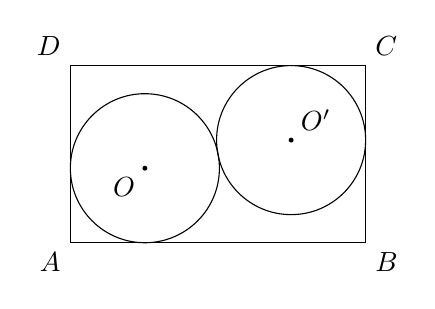
\begin{tikzpicture}[scale=0.75]
  \draw (0,0) rectangle (5,3);
  \node[below left] at (0,0) {$A$};
  \node[below right] at (5,0) {$B$};
  \node[above right] at (5,3) {$C$};
  \node[above left] at (0,3) {$D$};
  \draw (1.262,1.262) circle (1.262);
  \draw (3.738,1.738) circle (1.262);
  \fill (1.262,1.262) circle (1.2pt) node[below left] {$O$};
  \fill (3.738,1.738) circle (1.2pt) node[above right] {$O'$};
\end{tikzpicture}
\end{center}
\nopagebreak[4]
\gksubpart{附加题（2）正方体与球}

设两球半径为 $r,r'$，$s=r+r'$。两球心为 $(r,r,r)$ 与 $(1-r',1-r',1-r')$，外切条件变为

\nopagebreak[4]
\[\sqrt3(1-s)=s,\qquad s=\frac{\sqrt3}{1+\sqrt3}=\frac{3-\sqrt3}{2}\]

若考察两球体积和，

\nopagebreak[4]
\[V=\frac{4\pi}{3}(r^3+r'^3)=\frac{4\pi}{3}(s^3-3srr')\]

所以体积和最小时 $r=r'=s/2$；体积和最大时一个半径取 $1/2$，另一个取 $s-1/2=(2-\sqrt3)/2$，两者可交换。对应的体积最值分别由代入

\nopagebreak[4]
\[\left(r,r'\right)=\left(\frac{s}{2},\frac{s}{2}\right)\quad\text{\text{或}}\quad\left(\frac12,\frac{2-\sqrt3}{2}\right)\]

得到。
\nopagebreak[4]
\begin{center}% 1964 附加题（2）：正方体内两球的空间示意（矢量重绘）
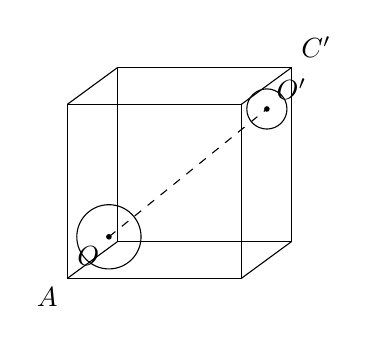
\begin{tikzpicture}[>=stealth,scale=0.85]
  \coordinate (A) at (0,0);
  \coordinate (B) at (2.6,0);
  \coordinate (C) at (2.6,2.6);
  \coordinate (D) at (0,2.6);
  \coordinate (Ap) at (0.75,0.55);
  \coordinate (Bp) at (3.35,0.55);
  \coordinate (Cp) at (3.35,3.15);
  \coordinate (Dp) at (0.75,3.15);
  \draw (A)--(B)--(C)--(D)--cycle;
  \draw (Ap)--(Bp)--(Cp)--(Dp)--cycle;
  \draw (A)--(Ap) (B)--(Bp) (C)--(Cp) (D)--(Dp);
  \draw (0.62,0.62) circle (0.48);
  \draw (2.98,2.53) circle (0.30);
  \fill (0.62,0.62) circle (1.2pt) node[below left] {$O$};
  \fill (2.98,2.53) circle (1.2pt) node[above right] {$O'$};
  \draw[dashed] (0.62,0.62)--(2.98,2.53);
  \node[below left] at (A) {$A$};
  \node[above right] at (Cp) {$C'$};
\end{tikzpicture}
\end{center}
\nopagebreak[4]
\gkanswer{答案（1）：$r+r'=2-\sqrt2$。}

\gkanswer{答案（2）：面积和最小时 $r=r'=\dfrac{2-\sqrt2}{2}$；面积和最大时 $(r,r')=\left(\dfrac12,\dfrac32-\sqrt2\right)$ 或交换两者。}

\end{answer}